%
% chapter.tex -- Beschreibung des Inhaltes
%
% (c) 2021 Prof Dr Andreas Müller, Hochschule Rapperswil
%
% !TeX spellcheck = de_CH
\chapter{Potenzen und Wurzeln
\label{buch:chapter:potenzen}}
\kopflinks{Potenzen und Wurzeln}
Die einfachsten Funktionen, die man allein mit den arithmetischen
Operationen definieren kann, sind Polynome der unabhängigen Variablen.
Die Einfachheit, mit der sich die Werte eines Polynoms berechnen lassen,
rechtfertigt natürlich nicht, dafür eine spezielle Funktion zu definieren.
Es gibt aber mindestens die folgenden drei wichtige Bereiche, in denen
Polynomen eine besondere Bedeutung zu kommt, die eine tiefergehende
Diskussion rechtfertigen.
\begin{enumerate}
\item
Die Umkehrfunktion der Potenzfunktion sind viel schwieriger zu 
\index{Potenzfunktion}%
berechnen und können als eine besonders einfache Art von speziellen
Funktionen betrachtet werden.
Die in Abschnitt~\ref{buch:potenzen:section:loesungen} definierten
Wurzelfunktionen sind der erste Schritt zur Lösung von Polynomgleichungen.
\index{Wurzelfunktion}%
\index{Polynomgleichung}%
\item
Es lassen sich interessante Familien von Funktionen
definieren, die zum Teil aus Polynomen bestehen.
Oft zeichnen sie sich durch Besonderheiten aus, die
direkt mit der Tatsache zusammenhängen, dass sie Polynome sind.
Die Tschebyscheff-Polynome als
Beispiel einer solchen Funktionenfamilie werden in
Abschnitt~\ref{buch:polynome:section:tschebyscheff} vorgestellt.
\item
Alle speziellen Funktionen sind analytisch, sie haben eine konvergente
Potenzreihenentwicklung.
\index{Potenzreihe}%
Die Partialsummen einer Potenzreihenentwicklung sind polynomielle
Approximationen dieser speziellen Funktionen.
An die wichtigsten Eigenschaften von Potenzreihen wird in 
Abschnitt~\ref{buch:potenzen:section:potenzreihen} erinnert.
\end{enumerate}

%
% 1-polynome.tex
%
% (c) 2021 Prof Dr Andreas Müller, OST Ostschweizer Fachhochschule
%
\section{Polynome
\label{buch:potenzen:section:polynome}}
\rhead{Polynome}
Die wohl einfachsten Funktionen, die sich mit den arithmetischen
Operationen konstruieren lassen, sind die Polynome.

\begin{definition}
\index{Polynom}%
Ein {\em Polynome} vom Grad $n$ ist die Funktion
\[
p(x) = a_nx^n + a_{n-1}x^{n-1} + \dots + a_2x^2 + a_1x + a_0,
\]
wobei $a_n\ne 0$ sein muss.
Das Polynom heisst {\em normiert}, wenn $a_n=1$ ist.
\index{normiert}%
\index{Grad eines Polynoms}%
\index{Polynom!Grad}%
Die Menge aller Polynome mit Koeffizienten in der Menge $K$ wird mit
$K[x]$ bezeichnet.
\end{definition}

Die Menge $K[x]$ ist heisst auch der {\em Polynomring}, weil $K[x]$
\index{Polynomring}%
mit der Addition, Subtraktion und Multiplikation von Polynomen eine
algebraische Struktur bildet, die man einen Ring mit $1$ nennt.
\index{Ring}%
Im Folgenden werden wir uns auf die Fälle $K=\mathbb{Q}$, $K=\mathbb{R}$
und $K=\mathbb{C}$ beschränken.

Für den Grad eines Polynoms gelten die bekannten Rechenregeln
\begin{align*}
\deg (a(x) + b(x)) &\le \operatorname{max}(\deg a(x), \deg b(x))
\\
\deg (a(x)\cdot b(x)) &=\deg a(x) + \deg b(x)
\end{align*}
für beliebige Polynome $a(x),b(x)\in K[x]$.

In Abschnitt~\ref{buch:orthogonalitaet:section:orthogonale-funktionen} werden
Familien von Polynomen konstruiert werden, die sich durch eine
Orthogonalitätseigenschaft auszeichnen.
Diese Polynome lassen sich typischerweise auch als Lösungen von
Differentialgleichungen finden.
Ausserdem werden hypergeometrische Funktionen
\[
\mathstrut_pF_q\biggl(
\begin{matrix}a_1,\dots,a_p\\b_1,\dots,b_q\end{matrix};z
\biggr),
\] die in
Abschnitt~\ref{buch:rekursion:section:hypergeometrische-funktion}
definiert werden, zu Polynomen, wenn mindestens einer der
Parameter $a_k$ negativ ganzzahlig ist.
Polynome sind also bereits eine vielfältige Quelle von speziellen
Funktionen.

Viele spezielle Funktionen werden aber komplizierter sein und
sich nicht als einfache Polynome ausdrücken lassen.
Genau diese Unmöglichkeit rechtfertigt ja, neue Funktionen
zu definieren.
Es bleibt aber immer noch die Notwendigkeit, effiziente 
Berechnungsverfahren für die speziellen Funktionen zu konstruieren.
Dank des folgenden Satzes kann dies immer mit Polynomen geschehen.

\begin{satz}[Weierstrass]
\index{Satz!Weierstrass}%
\index{Weierstrasse, Karl}%
\label{buch:potenzen:satz:weierstrass}
\index{Weierstrass, Satz von}%
Eine auf einem kompakten Intervall $[a,b]$ stetige Funktion $f(x)$
lässt sich durch eine Folge $p_n(x)$ von Polynomen gleichmässig
approximieren.
\end{satz}

Der Satz sagt in dieser Form nichts darüber aus, wie die
Approximationspolynome konstruiert werden sollen.
\index{Approximationspolynom}%
Von Bernstein gibt es konstruktive Beweise dieses Satzes,
\index{Bernstein-Polynom}%
welche auch explizit eine Folge von Approximationspolynomen
konstruieren.
In der späteren Entwicklung werden wir für die meisten
speziellen Funktionen Potenzreihen entwickeln, deren Partialsummen
ebenfalls als Approximationen dienen können.
Weitere Möglichkeiten liefern Interpolationsmethoden der
numerischen Mathematik.

Diese Betrachtungsweise von Polynomen als Funktionen trägt
aber den zusätzlichen algebraischen Eigenschaften des Polynomringes
nicht ausreichend Rechnung.
Zum Beispiel bedeutet Gleichheit von zwei reellen Funktion $f(x)$ und
$g(x)$, dass man $f(x)=g(x)$ für alle $x\in\mathbb{R}$ nachprüfen
muss.
Für Polynome reicht es jedoch, die Funktionswerte in nur wenigen
Punkten zu vergleichen.
Dies äussert sich zum Beispiel auch im Prinzip des
Koeffizientenvergleichs von
Satz~\ref{buch:polynome:satz:koeffizientenvergleich}.
Im Gegensatz zu beliebigen Funktionen kann man daher Aussagen
über Polynomen immer mit endlich Algorithmen entscheiden.
Die nächsten Abschnitte sollen diese algebraischen Eigenschaften
zusammenfassen.

%
% Polynomdivision, Teilbarkeit und ggT
%
\subsection{Polynomdivision, Teilbarkeit und grösster gemeinsamer Teiler}
Der schriftliche Divisionsalgorithmus für Zahlen funktioniert 
auch für die Division von Polynomen.
\index{Polynome!Divisionsalgorithmus}%
Zu zwei beliebigen Polynomen $p(x)$ und $q(x)$ lassen sich also
immer zwei Polynome $a(x)$ und $r(x)$ finden derart, dass
$p(x) = a(x) q(x) + r(x)$.
Das Polynom $a(x)$ heisst der {\em Quotient}, $r(x)$ der {\em Rest}
der Division.
Das Polynom $p(x)$ heisst {\em teilbar} durch $q(x)$, geschrieben
\index{teilbar}%
\index{Polynome!teilbar}%
$q(x)\mid p(x)$, wenn $r(x)=0$ ist.

%
% Grösster gemeinsamer Teiler
%
\subsubsection{Grösster gemeinsamer Teiler}
Mit dem Begriff der Teilbarkeit geht auch die Idee des grössten
gemeinsamen Teilers einher.
Ein gemeinsamer Teiler zweier Polynome $a(x)$ und $b(x)$ 
\index{gemeinsamer Teiler}%
ist ein Polynom $g(x)$, welches beide Polynome teilt, also
$g(x)\mid a(x)$ und $g(x)\mid b(x)$.
\index{grösster gemeinsamer Teiler}%
\index{Polynome!grösster gemeinsamer Teiler}%
Ein Polynom $g(x)$ heisst {\em grösster gemeinsamer Teiler} von $a(x)$
und $b(x)$, wenn jeder andere gemeinsame Teiler $f(x)$ von $a(x)$
und $b(x)$ auch ein Teiler von $g(x)$ ist.
Man beachte, dass die skalaren Vielfachen eines grössten gemeinsamen
Teilers ebenfalls grösste gemeinsame Teiler sind, der grösste gemeinsame
Teiler ist also nicht eindeutig bestimmt.

%
% Der euklidische Algorithmus
%
\subsubsection{Der euklidische Algorithmus}
\index{Algorithmus!euklidisch}%
\index{euklidischer Algorithmus}%
Zur Berechnung eines grössten gemeinsamen Teilers steht wie bei den
ganzen Zahlen der euklidische Algorithmus zur Verfügung.
Dazu bildet man die Folgen von Polynomen
\[
\begin{aligned}
a_0(x)&=a(x) & b_0(x) &= b(x)
&
&\Rightarrow&
a_0(x)&=b_0(x) q_0(x) + r_0(x) &&
\\
a_1(x)&=b_0(x) & b_1(x) &= r_0(x)
&
&\Rightarrow&
a_1(x)&=b_1(x) q_1(x) + r_1(x) &&
\\
a_2(x)&=b_1(x) & b_2(x) &= r_1(x)
&
&\Rightarrow&
a_2(x)&=b_2(x) q_2(x) + r_2(x) &&
\\
&&&&&\hspace*{2mm}\vdots&&
\\
a_{m-1}(x)&=b_{m-2}(x) & b_{m-1}(x) &= r_{m-2}(x) 
&
&\Rightarrow&
a_{m-1}(x)&=b_{m-1}(x)q_{m-1}(x) + r_{m-1}(x) &\text{mit }r_{m-1}(x)&\ne 0
\\
a_m(x)&=b_{m-1}(x) & b_m(x)&=r_{m-1}(x)
&
&\Rightarrow&
a_m(x)&=b_m(x)q_m(x).&&
\end{aligned}
\]
Der Index $m$ ist der Index, bei dem zum ersten Mal $r_m(x)=0$ ist.
Dann ist $g(x)=r_{m-1}(x)$ ein grösster gemeinsamer Teiler.

%
% Der erweiterte euklidische Algorithmus
%
\subsubsection{Der erweiterte euklidische Algorithmus}
\index{Polynome!erweiterter euklidischer Algorithmus}%
\index{erweiterter euklidischer Algorithmus}%
\index{euklidischer Algorithmus!erweitert}%
Die Konstruktion der Folgen $a_n(x)$ und $b_n(x)$ kann in Matrixform
kompakter geschrieben werden als
\[
\begin{pmatrix}
a_k(x)\\
b_k(x)
\end{pmatrix}
=
\begin{pmatrix}
b_{k-1}(x)\\
r_{k-1}(x)
\end{pmatrix}
=
\begin{pmatrix}
0 & 1\\
1 & -q_{k-1}(x)
\end{pmatrix}
\begin{pmatrix}
a_{k-1}(x)\\
b_{k-1}(x)
\end{pmatrix}.
\]
Kürzen wir die $2\times 2$-Matrix als
\[
Q_k(x) = \begin{pmatrix} 0&1\\1&-q_k(x)\end{pmatrix}
\]
ab, dann ergibt das Produkt der Matrizen $Q_0(x)$ bis $Q_{m}(x)$
\[
\begin{pmatrix}
g(x)\\
0
\end{pmatrix}
=
\begin{pmatrix}
r_{m-1}(x)\\
r_{m}(x)
\end{pmatrix}
=
Q_{m}(x)
Q_{m-1}(x)
\cdots
Q_1(x)
Q_0(x)
\begin{pmatrix}
a(x)\\
b(x)
\end{pmatrix}.
\]
Zur Berechnung des Produktes der Matrizen $Q_k(x)$ kann man rekursiv
vorgehen mit der Rekursionsformel
\[
S_{k}(x) = Q_{k}(x) S_{k-1}(x)
\qquad\text{mit}\qquad
S_{-1}(x)
=
\begin{pmatrix} 1 & 0 \\ 0 & 1 \end{pmatrix}.
\]
Ausgeschrieben bedeutet dies Matrixrekursionsformel
\[
S_{k-1}(x)
=
\begin{pmatrix} 
c_{k-1} & d_{k-1} \\
c_k     & d_k
\end{pmatrix}
\qquad\Rightarrow\qquad
Q_{k}(x) S_{k-1}(x)
=
\begin{pmatrix}
0&1\\1&-q_k(x)
\end{pmatrix}
\begin{pmatrix} 
c_{k-1} & d_{k-1} \\
c_k     & d_k
\end{pmatrix}
=
\begin{pmatrix}
c_k&d_k\\
c_{k+1}&d_{k+1}
\end{pmatrix}.
\]
Daraus lässt sich für die Matrixelemente die Rekursionsformel
\[
\begin{aligned}
c_{k+1} &= c_{k-1} - q_k(x) c_k(x) \\
d_{k+1} &= d_{k-1} - q_k(x) d_k(x)
\end{aligned}
\quad
\bigg\}
\qquad
\text{mit Startwerten}
\qquad
\bigg\{
\begin{aligned}
\quad
c_{-1} &= 1, & c_0 &= 0 \\
d_{-1} &= 0, & d_0 &= 1.
\end{aligned}
\]
Wendet man die Matrix $S_m(x)$ auf den Vektor mit den Komponenten
$a(x)$ und $b(x)$, erhält man die Beziehungen
\[
g(x) = c_{k-1}(x) a(x) + d_{k-1}(x) b(x)
\qquad\text{und}\qquad
0 = c_k(x) a(x) + d_k(x) b(x).
\]
Dieser Algorithmus heisst der erweiterte euklidische Algorithmus.
Wir fassen die Resultate zusammen im folgenden Satz.

\begin{satz}
Zu zwei Polynomen $a(x),b(x) \in K[x]$ gibt es Polynome
$g(x),c(x),d(x)\in K[x]$
derart, dass $g(x)$ ein grösster gemeinsamer Teiler von $a(x)$ und $b(x)$
ist, und ausserdem
\[
g(x) = c(x)a(x)+d(x)b(x)
\]
gilt.
\end{satz}

%
% Faktorisierung und Nullstellen
%
\subsection{Faktorisierung und Nullstellen
\label{buch:polynome:subsection:faktorisierung-und-nullstellen}}
% wird später gebraucht um bei der Definition der hypergeometrischen Reihe
% die Zaehler- und Nenner-Polynome als Pochhammer-Symbole zu entwickeln
Ist $\alpha$ eine Nullstelle des Polynoms $a(x)$, also $a(\alpha)=0$.
Der Divisionsalgorithmus mit für die Polynome $a(x)$ und $b(x)=x-\alpha$
liefert zwei Polynome $q(x)$ für den Quotienten und $r(x)$ für den Rest
mit den Eigenschaften
\[
a(x)
=
q(x) b(x)
+r(x)
=
q(x)(x-\alpha)+r(x)
\qquad\text{mit}\qquad
\deg r < \deg b(x)=1.
\]
Der Rest $r(x)$ ist somit eine Konstante. 
Setzt man $x=\alpha$ ein, folgt
\[
0
=
a(\alpha)
=
q(\alpha)(\alpha-\alpha)+r(\alpha)
=
r(\alpha),
\]
der Rest $r(x)$ muss also verschwinden.
Für eine Nullstelle $\alpha$ von $a(x)$ ist $a(x)$ durch $(x-\alpha)$
teilbar.
Daraus folgt auch, dass ein Polynom $a(x)$ vom Grad $n=\deg a(x)$ höchstens
$n$ verschiedene Nullstellen haben kann.

Sind $\alpha_1,\dots,\alpha_k$ alle Nullstellen von $a(x)$, dann lässt
sich $a(x)$ zerlegen in Faktoren
\[
a(x)
=
(x-\alpha_1)^{m_1}
(x-\alpha_2)^{m_2}
\cdots
(x-\alpha_k)^{m_k}
b(x).
\]
Das Polynom $b(x)\in K[x]$ hat keine Nullstellen in $K$.

Wenn zwei Polynome $a(x)$ und $b(x)$ eine gemeinsame Nullstelle $\alpha$
haben, dann ist $(x-\alpha)$ ein Teiler beider Polynome und somit auch
ein Teiler eines grössten gemeinsamer Teiler.
Insbesondere sind die Nullstellen des grössten gemeinsamen Teilers
gemeinsame Nullstellen von $a(x)$ und $b(x)$.

%
% Koeffizienten-Vergleich
%
\subsection{Koeffizienten-Vergleich}
% Wird gebraucht für die Potenzreihen-Methode
% Muss später ausgedehnt werden auf Potenzreihen
Wenn zwei Polynome $a(x)$ und $b(x)$ vom Grad $\le n$ die gleichen
Koeffizienten haben, dann sind sie selbstverständlich gleich.
Weniger klar ist, ob zwei Polynome, die die gleichen Werte für beliebige
$x$ haben, auch die gleichen Koeffizienten haben.
Wir nehmen also an, dass $a(x)=b(x)$ gilt für jedes $x\in K$ und
wollen daraus ableiten, dass die Koeffizienten übereinstimmen müssen.
Seien $x_1,\dots,x_n$ verschiedene Elemente in $K$, dann
hat das Polynom $p(x)=a(x)-b(x)$, welches Grad $\le n$ hat,
die $n$ Nullstellen $x_k$ für $k=1,\dots,n$.
$p(x)$ ist also durch alle Polynome $x-x_k$ teilbar.
Weil $\deg p\le n$ ist, muss 
\[
0
=
a(x)-b(x)
=
p(x)
=
p_n
(x-x_1)(x-x_2)\cdots (x-x_n)
\]
sein.
Ist $y\in K$ verschieden von den Nullstellen $x_i$, dann ist 
in $y-x_i\ne 0$ für alle $i$.
Für das Produkt gilt dann
\[
0
=
p(y) 
=
p_n
(\underbrace{x-x_1}_{\displaystyle \ne 0})
\cdots
(\underbrace{x-x_n}_{\displaystyle \ne 0}),
\]
so dass $p_n=0$ sein muss, was schliesslich dazu führt, dass alle
Koeffizienten von $a(x)-b(x)$ verschwinden.
Daraus folgt das Prinzip des Koeffizientenvergleichs:
\index{Koeffizientenvergleich}%
\index{Polynome!Koeffizientenvergleich}%

\begin{satz}[Koeffizientenvergleich]
\index{Satz!Koeffizientenvergleich}%
\label{buch:polynome:satz:koeffizientenvergleich}
Zwei Polynome $a(x)$ und $b(x)$ stimmen genau dann überein, wenn
sie die gleichen Koeffizienten haben.
\end{satz}

Man beachte, dass dieses Prinzip nur funktioniert, wenn es genügend
viele verschiedene Elemente in $K$ gibt.
Für die endlichen Körper $\mathbb{F}_p$ gilt dies nicht, denn es gilt
\[
a(x)
=
x^p-x\equiv 0\mod p
\]
für jede Zahl $x\in\mathbb{F}_p$, das Polynom $a(x)$ mit Grad $p$
hat also genau $p$ Nullstellen, es gibt aber keine weitere Nullstelle,
mit der man wie oben schliessen könnte, dass $a(x)$ das Nullpolynom ist.

%
% Berechnung von Polynom-Werten
%
\subsection{Berechnung von Polynom-Werten}
Die naive Berechnung der Werte eines Polynoms $p(x)$ vom Grad $n$
beginnt mit der Berechnung der Potenzen von $x$.
Da alle Potenzen benötigt werden, wird man dazu $n-1$ Multiplikationen
benötigen.
Die Potenzen müssen anschliessend mit den Koeffizienten multipliziert
werden, dazu sind weitere $n$ Multiplikationen nötig.
Der Wert des Polynoms kann also erhalten werden mit $2n-1$ Multiplikationen
und $n$ Additionen.

Die Anzahl nötiger Multiplikationen kann mit dem folgenden Vorgehen
reduziert werden, welches auch als das {\em Horner-Schema} bekannt ist.
\index{Horner-Schema}%
\index{Polynome!Horner-Schema}%
Statt erst am Schluss alle Terme zu addieren, addiert man so früh
wie möglich.
Zum Beispiel multipliziert man $(a_nx+a_{n-1})$ mit $x$, was auf
die Multiplikationen beider Terme mit $x$ hinausläuft.
Mit dieser Idee kann man das Polynom als
\[
a_nx^n
+
a_{n+1}x^{n+1}
+
\dots
+
a_1x
+
a_0
=
((\dots((a_nx+a_{n-1})x+a_{n-2})x+\dots )x+a_1)x+a_0
\]
schreiben.
Beginnend bei der innersten Klammer sind genau $n$ Multiplikationen
und $n$ Additionen nötig, man spart mit diesem Vorgehen also
$n-1$ Multiplikationen. 




%
% 2-loesbarkeit.tex
%
% (c) 2021 Prof Dr Andreas Müller, OST Ostschweizer Fachhochscule
%
\section{Lösungen von Polynomgleichungen
\label{buch:potenzen:section:loesungen}}
\kopfrechts{Lösungen von Polynomgleichungen}
Die Berechnung von Polynomen ist sehr einfach, da nur arithmetische 
Grundoperationen benötigt werden.
In vielen Anwendungen sind jedoch die Argumente gefragt, für die ein
Polynom einen bestimmten Wert annimmt.
Es geht also um die Lösung von Gleichungen der Form
\[
p(x) = c
\]
für ein Polynome $p(x)$ und eine Konstante $c\in\mathbb{C}$.

%
% Fundamentalsatz der Algebra
%
\subsection{Fundamentalsatz der Algebra}
In Abschnitt~\ref{buch:polynome:subsection:faktorisierung-und-nullstellen}
wurde gezeigt, dass sich jede Nullstellen $\alpha$ eines Polynoms als
Faktor $x-\alpha$ abspalten lässt.
Jedes Polynom liess sich in ein Produkt von Linearfaktoren und
einen Faktor zerlegen, der keine Nullstellen hat.
Zum Beispiel hat das Polynom $x^2+1\in\mathbb{R}[x]$ keine
Nullstellen in $\mathbb{R}$.
Eine solche Nullstelle müsste eine Quadratwurzel von $-1$ sein.
Die komplexen Zahlen $\mathbb{C}$ wurden genau mit dem Ziel konstruiert,
dass $i=\sqrt{-1}$ sinnvoll wird.
Der Fundamentalsatz der Algebra zeigt, dass $\mathbb{C}$ alle
Nullstellen von Polynomen enthält.

\begin{satz}[Gauss]
\index{Satz!Fundamentalsatz der Algebra}%
\index{Fundamentalsatz der Algebra}%
\label{buch:potenzen:satz:fundamentalsatz}
Jedes Polynom $p(x)=a_nx^n+\dots + a_2x^2 + a_1x + a_0\in\mathbb{C}[x]$
zerfällt in ein Produkt
\[
p(x)
=
a_n
(x-\alpha_1)(x-\alpha_2)\cdots(x-\alpha_n)
\]
für Nullstellen $\alpha_k\in\mathbb{C}$.
\end{satz}


%
% Lösbarkeit durch Wurzelausdrücke
%
\subsection{Lösbarkeit durch Wurzelausdrücke}
Der Fundamentalsatz macht keine Aussage darüber, wie die Nullstellen
eines Polynoms gefunden werden können.
Selbst für besonders einfache Gleichungen der Form
\(
x^n = c
\)
oder gleichbedeutend die Bestimmung der Nullstellen von Polynomen der Form
\(
p(x) = x^n -c
\)
gibt es für $n>1$ im Allgemeinen keine direkte, nur auf den arithmetischen
Grundoperationen basierende Methode, eine Lösung oder Faktorisierung
in endlich vielen Schritten zu finden.
Dies rechtfertigt, für diese einfachen Fälle eine neue, spezielle
Funktion zu definieren, die mindestens für reelle Koeffizienten 
die Nullstelle als Rückgabewert hat.

\begin{figure}
\centering
\includegraphics{chapters/010-potenzen/images/wurzel.pdf}
\caption[Graph der Wurzelfunktionen]{Graph der Wurzelfunktionen
\ensuremath{x\mapsto\root{n}\of{x}}
als Umkehrfunktionen der Potenzfunktionen $x\mapsto x^n$ für
$n=2$ ({\color{red}rot}), $n=3$ ({\color{blue}blau}),
$n=16$ ({\color{darkgreen}grün}) und $n=27$ ({\color{orange}orange}).
\label{buch:potenzen:fig:wurzel}
}
\end{figure}

\begin{definition}
Die inverse Funktion der Potenzfunktion
$f\colon \mathbb{R}\to\mathbb{R}:x\mapsto y=f(x)=x^n$
heisst die $n$-{\em te Wurzel} und wird
\[
\root{n}\of{\mathstrut\phantom{m}}
=
f^{-1}
\colon
D\to\mathbb{R}
:
y\mapsto f^{-1}(y)=\root{n}\of{\mathstrut y}
\]
geschrieben.
Für gerades $n$ ist der Definitionsbereich der Wurzel nur
$D=\mathbb{R}_{\ge 0}$, für ungerades $n$ ist $D=\mathbb{R}$.
Für $n=2$ wird die Wurzel als
\(
\root{2}\of{\mathstrut y}
=
\sqrt{\mathstrut y}
\)
geschrieben.
\end{definition}

Mit Hilfe der Wurzelfunktion ist es jetzt möglich, auch kompliziertere
Gleichungen zu lösen:
\begin{enumerate}
\item
Die quadratische Gleichung 
\[
ax^2+bx+c=0
\]
hat die Nullstellen
\begin{equation}
x_{1,2} = \frac{-b\pm\sqrt{b^2-4ac\mathstrut}}{2a}.
\label{buch:potenzen:eqn:quadrgl}
\end{equation}
\item
Für kubische Gleichungen hat Cardano eine Lösung gefunden, die
Nur Wurzelausdrücke und arithmetische Operationen verwendet.
Die Gleichung $x^3+px+q=0$ hat die Nullstelle
\[
x
=
\root{3}\of{-\frac{q}2+\sqrt{\frac{q^2}4+\frac{p^3}{27}}}
+
\root{3}\of{-\frac{q}2-\sqrt{\frac{q^2}4+\frac{p^3}{27}}}.
\]
Falls das Argument der Quadratwurzel negativ ist, muss eine
Kubikwurzel aus einer komplexen Zahl berechnet werden, was
wieder über die Möglichkeiten der oben definierten Wurzelfunktionen
hinausgeht.
\item
Für die Lösung einer Gleichung vierten Grades hat Ferrari eine
Formel angegeben, die mit Wurzelausdrücken und arithmetischen
Operationen auskommt.
\item
Für negative Argument $y<0$ müssen Quadratwurzeln als
$\sqrt{y\mathstrut}=i\sqrt{-y\mathstrut}$ definiert werden.
Damit wird auch für $b^2-4ac<0$ sinnvoll.
\eqref{buch:potenzen:eqn:quadrgl}
\item
Mindestens der Betrag der Wurzel einer komplexen Zahl lässt
sich nun auch mittels $|\root{n}\of{c\mathstrut}|=\root{n}\of{|c|\mathstrut}$
berechnen.
Für das Argument sind jedoch die in
Abschnitt~\label{buch:geometrie:section:trigonometrisch} definierten
trigonometrischen Funktionen notwendig.
\end{enumerate}

Allerdings ist damit auch bereits ausgeschöpft, was die
Wurzelfunktionen zur Lösung von Polynomgleichungen beitragen
können.
Der folgende Satz von Abel zeigt, dass man für Polynomgleichungen
höheren Grades nicht mit einer Lösung durch Wurzelausdrücke
rechnen kann.

\begin{satz}[Abel]
\index{Satz!von Abel}
\label{buch:potenzen:satz:abel}
Für Polynomgleichungen vom Grad $n\ge 5$ gibt es keine allgemeine
Lösung durch Wurzelausdrücke.
\end{satz}



%
% Algebraische Zahlen
%
\subsection{Algebraische Zahlen}
Die Verwendung der komplexen Zahlen ist für numerische Rechnungen
zweckmässig.
In den Anwendungen der Computer-Algebra hingegen erwartet man zum
Beispiel exakte Formeln für eine Stammfunktion.
\index{Computer-Algebra}%
\index{CAS}%
Nicht rationale Zahlen können nur exakt verarbeitet werden, wenn
Sie sich algebraisch in endlich vielen Schritten charakterisieren
lassen.
Dies ist zum Beispiel für rationale Zahlen $\mathbb{Q}$ möglich.
Gewisse irrationale Zahlen kann man durch die Eigenschaft charakterisieren,
Nullstelle eines Polynoms $p(x)\in\mathbb{Q}[x]$
mit rationalen Koeffizienten zu sein.

\begin{definition}
Eine Zahl $\alpha$ heisst {\em algebraisch} über $\mathbb{Q}$,
wenn es ein Polynom
\index{algebraische Zahl}%
$p(x)\in \mathbb{Q}[x]$ gibt, welches $\alpha$ als Nullstelle hat.
Eine Zahl heisst transzendent über $\mathbb{Q}$, wenn sie nicht algebraisch
über $\mathbb{Q}$ ist.
\end{definition}

Die Zahlen $i=\sqrt{-1}$ und $\sqrt{n\mathstrut}$ für $n\in\mathbb{N}$
sind also algebraisch über $\mathbb{Z}$.
Euler und Lambert konnten zeigen, dass $e$ und $\pi$ irrational sind,
Hermite bzw.~Lindemann konnten sogar zeigen, dass sie transzendent sind.

Eine Polynomgleichung $p(\alpha)=0$ mit $p(x)\in\mathbb{Q}[x]$
hat eine Rechenregel für $\alpha$ zur Folge.
Dazu schreibt man
\[
p_n\alpha^n + p_{n-1}\alpha^{n-1} + \dots + a_1\alpha + a_0 =0
\qquad\Rightarrow\qquad
\alpha^n = -\frac{1}{p_n}\bigl(
p_{n-1}\alpha^{n-1}+\dots+a_1\alpha+a_0
\bigr).
\]
Diese Regel erlaubt, jede Potenz $\alpha^k$ mit $k\ge n$ durch
Potenzen von $\alpha^l$ mit $l<n$ auszudrücken.
Die Zahlen, die sich durch arithmetische Operationen aus
$\alpha$ bilden lassen, lassen sich also sogar durch lineare
Operationen aus $1,\alpha,\alpha^2,\dots,\alpha^{n-1}$
bilden.
Sie bilden einen endlichdimensionalen Vektorraum über $\mathbb{Q}$.
Rechnen mit algebraischen Zahlen ist also in einem CAS exakt möglich,
wie das in Abschnitt~\ref{buch:integrale:section:dkoerper}
für die Berechnung von Stammfunktionen illustriert werden wird.



%
% 3-tschebyscheff.tex
%
% (c) 2021 Prof Dr Andreas Müller
%
\section{Die Tschebyscheff-Polynome
\label{buch:polynome:section:tschebyscheff}}
Die Tschbeyscheff-Polynome sind ein Beispiel einer nützlichen Familie
von Polynomen, die wegen ihrer Anwendbarkeit durchaus den Rang von
speziellen Funktionen im weiteren Sinne verdienen.
Sie ermöglichen, Interpolationspolynome mit besonders guten
Fehlereigenschaften zu finden, haben aber auch andere Anwendungen
zum Beispiel beim Design von Filtern in der Elektronik.

%
% Motivation: Interpolation
%
\subsection{Motivation: Interpolation}
Nach dem Satz von Weierstrass
(Satz~\ref{buch:potenzen:satz:weierstrass})
lässt sich jede stetige Funktion auf einem kompakten Intervall durch
ein Polynom approximieren.
Interpolation kann zur Konstruktion solcher approximierender Polynome
verwendet werden, wie die folgenden Abschnitte zeigen sollen.
Die Optimierung des Approximationsfehlers führt auf die Spezifikation
einer interessanten Familie von Polynomen.

%
% Lagrange-Interpolationspolynom
%
\subsubsection{Lagrange-Interplationspolynom}
Eine mögliche Lösung des Problems, solche approximierenden Polynome
der Funktion $f(x)$
zu finden, besteht darin, ein Polynom $p(x)$ zu konstruieren, welches
in einzelnen, Stützstellen genannten Werten $x_0<x_1<\dots<x_n$ der
unabhängigen Variablen mit $f$ übereinstimmt, also
\[
p(x_i) = f(x_i), \quad i=0,\dots,n.
\]
Die Konstruktion eines solchen Polynoms geht aus vom Polynom
\[
l(x) = (x-x_0)(x-x_1)\cdots(x-x_n),
\]
welches an allen Stützstellen verschwindet.
Daraus lässt sich für jede Stützstelle ein Polynom
\[
l_j(x)
=
\frac{
(x-x_0)(x-x_1)\cdots\widehat{(x-x_j)}\cdots(x-x_n)
}{
(x_j-x_0)(x_j-x_1)\cdots\widehat{(x_j-x_j)}\cdots(x_j-x_n)
}
\]
konstruieren, wobei $\widehat{(x-x_j)}$ bedeutet, dass dieser Faktor
weggelassen werden soll.
Das Polynom $l_j(x)$ hat die Werte
\begin{align}
l_j(x_k)
&=
\frac{
(x_k-x_0)(x_k-x_1)\cdots\widehat{(x_k-x_j)}\cdots(x_k-x_n)
}{
(x_j-x_0)(x_j-x_1)\cdots\widehat{(x_j-x_j)}\cdots(x_j-x_n)
}
=
\delta_{jk}
=
\begin{cases}
1&\qquad j=k\\
0&\qquad j\ne k
\end{cases}
\label{buch:potenzen:interpolation:lj}
\end{align}
auf den Stützstellen.
Für $j\ne k$ enthält der Zähler von $l_j(x_k)$ den Faktor
$(x-x_k)$, der für $x=x_k$ verschwindet.
Daher verschwindet auch $l_j(x)$ für $x=x_k$.

\index{Lagrange-Interpolationspolynom}%
Das sogenannte {\em Lagrange-Interpolationspolynom} ist das Polynom
\[
p(x)
=
\sum_{j=0}^n f(x_j) l_j(x).
\]
Aus der Eigenschaft~\eqref{buch:potenzen:interpolation:lj} folgt, dass
\[
p(x_k)
=
\sum_{j=0}^n f(x_j) l_j(x_k)
=
\sum_{j=0}^n f(x_j) \delta_{jk}
=
f(x_k).
\]

%
% Fehler des Interpolationspolynoms
%
\subsubsection{Fehler des Interpolationspolynoms}
Der Approximationsfehler des Interpolationspolynoms kann mit der Formel
\[
f(x)-p(x)
=
l(x) \frac{f^{(n+1)}(\xi)}{(n+1)!}
\]
für einen geeigneten Wert $\xi$ mit $x_0 < \xi < x_n$.
Über die Ableitungen hat man natürlich keine Kontrolle, die einzige 
Möglichkeit, den Fehler möglichst klein zu halten ist daher,
die Sütztstellen so zu wählen, dass $l(x)$ kleine Funktionswerte hat.
Stützstellen in gleichen Abständen erweisen sich dafür als ungeeignet,
da $l(x)$ nahe $x_0$ und $x_n$ sehr stark oszilliert.

%
% Definition Tschbeyscheff-Polynome
%
\subsection{Definition der Tschebyscheff-Polynome
\label{sub:definiton_der_tschebyscheff-Polynome}}
\begin{figure}
\centering
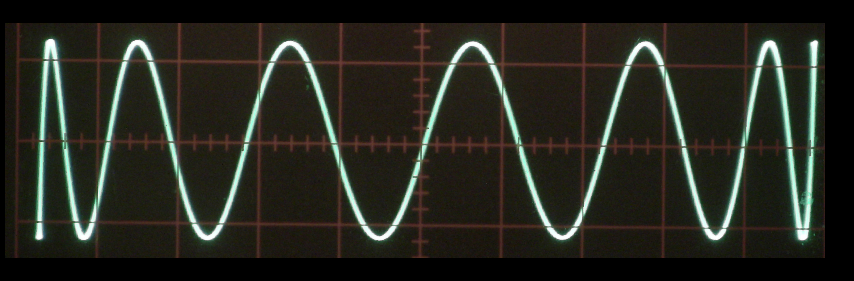
\includegraphics[width=\textwidth]{chapters/010-potenzen/images/lissajous.pdf}
\caption{Lissajous-Figur für zwei Signale $x=\cos t$ und $y=\cos 12t$.
\label{buch:potenzen:interpolation:lissajous}}
\end{figure}
\begin{figure}
\centering
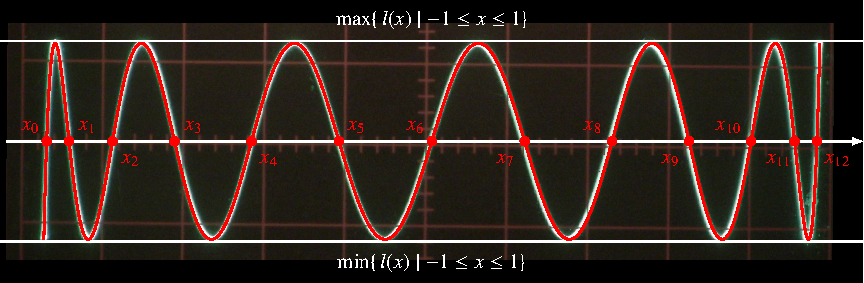
\includegraphics[width=\textwidth]{chapters/010-potenzen/images/lissajous-chebyshef.pdf}
\caption{Das Tschebyscheff-Polynom als Lösung des Interpolationsproblems.
\label{buch:potenzen:interpolation:lissajous-tschebyscheff}}
\end{figure}
Die Aufgabe, geeignete Stützstellen für das Interpolationsproblem zu finden,
die den Fehler minimieren, ist als gleichbedeutend damit, ein Polynom
zu finden, dessen Betrag beschränkt ist.
Eine Lissajous-Figur wie die in
Abbildung~\ref{buch:potenzen:interpolation:lissajous} erfüllt
diese Bedinung.
Sofern sie sich als Polynom ausdrücken lässt, könnte ihre Nullstellen
das Interpolationsproblem optimal lösen.

In der Lissajous-Figur in
Abbildung~\ref{buch:potenzen:interpolation:lissajous} ist
die Funktion $x=\cos t$ und $y=\cos 12t$ dargestellt.
Wegen $t=\arccos x$
Als Funktion von $x$ ist daher
\[
y(x) = \cos(nt)=\cos(n\arccos x).
\]
Tatsächlich ist aus der Theorie der trigonometrischen Funktionen
bekannt, dass die Kosinus eines Vielfachen des Winkels immer
als Polynom des Kosinus des Winkels dargestellt werden können.

\begin{definition}
\index{Tschebyscheff-Polynome}%
\label{buch:potenzen:def:tschebyscheff}
Das Polynom
\[
T_n(x)
=
\cos (n\arccos x),
\qquad
x\in[-1,1]
\]
heisst
{\em Tschebyscheff-Polynom (erster Art)} vom Grad $n$.
\end{definition}
Die Tschebyscheff-Polynome eignen sich auch hervorragend
dafür, Eigenschaften spezieller Funktionenfamilien zu
illustrieren.
Es wird sich zeigen, dass die Tschebyscheff-Polynome
Lösungen einer speziellen Differentialgleichung sind und
bezüglich eines in Kapitel~\ref{buch:chapter:orthogonalitaet}
definierten Skalarproduktes von Funktionen orthonormiert sind.

%
% Rekursionsbeziehungen
%
\subsection{Rekursionsbeziehungen
\label{buch:potenzen:tschebyscheff:rekursionsbeziehungen}}
Es ist etwas mühsam, einen Ausdruck von $T_n(x)$ direkt aus
trigonometrischen Identitäten herzuleiten.
In diesem Abschnitt soll daher eine Rekursionsbeziehung
hergeleitet werden.
Später in Abschnitt~\ref{buch:orthogonal:section:drei-term-rekursion}
wird gezeigt, dass solche Rekursionsbeziehungen eine Begleiterscheinung
orthogonaler Polynome sind.

%
% Drei-Term-Rekursion für die Tschebyscheff-Polynome
%
\subsubsection{Drei-Term-Rekursion für die Tschebyscheff-Polynome}
Mit der Abkürzung $y=\arccos(x)$ oder $x=\cos(y)$ bekommt man aus
der Definition~\label{buch:potenzen:def:tschebyscheff}
der Tschebyscheff-Polynome
\index{Drei-Term-Rekursion!für Tschebyscheff-Polynome}
\begin{align*}
xT_n(x)
&=
\cos(y)\cdot \cos(ny)
\\
&=
\frac12\bigl(
\cos((n+1)y) + \cos((n-1)y)
\bigr)
\\
x\,T_n(x)
&=
\frac12 T_{n+1}(x) + \frac12 T_{n-1}(x).
\end{align*}
Auflösen nach $T_{n+1}(x)$ ergibt
\begin{equation}
T_{n+1}(x) = 2x\,T_n(x)-T_{n-1}(x),
\quad
\text{mit Startwerten}
\quad T_1(x)=x,
\quad
T_0(x)=1.
\label{buch:potenzen:tschebyscheff:eqn:rekursion}
\end{equation}
Damit können die Tschebyscheff-Polynome sehr effizient berechnet werden:
\begin{equation}
\label{eq:tschebyscheff-polynome}
\begin{aligned}
T_0(x)
&=1
\\
T_1(x)
&=
x
\\
T_2(x)
&=
2x^2-1
\\
T_3(x)
&=
4x^3-3x
\\
T_4(x)
&=
8x^4-8x^2+1
\\
T_5(x)
&=
16x^5-20x^3+5x
\\
T_6(x)
&=
32x^6-48x^4+18x^2-1
\\
T_7(x)
&=
64x^7-112x^5+56x^3-7x
\\
T_8(x)
&=
128x^8-256x^6+160x^4-32x^2+1
\end{aligned}
\end{equation}
Die Rekursionsformel~\eqref{buch:potenzen:tschebyscheff:eqn:rekursion}
kann auch dazu verwendet werden, Werte der Tschebyscheff-Polynome
zu berechnen, wie in Übungsaufgabe~\ref{104} gezeigt wird.
Für $|x|>\frac12$ wird bei jeder Anwendung der Rekursion mit dem
Faktor $|2x|>1$ multipliziert.
Eventuell vorhandene Rundungsfehler werden natürlich ebenfalls
multipliziert und es besteht die Gefahr, dass diese exponentiell
schnell anwachsen.
Die Rechnung in Übungsaufgabe~\ref{104} zeigt aber, dass die
Resultate stabil auch für $n \approx 10^5$.

%
% Drei-Term-Rekursion für die Ableitung
%
\subsubsection{Drei-Term-Rekursion für die Ableitung}
Durch Ableitung der 
Rekursionsformel~\eqref{buch:potenzen:tschebyscheff:eqn:rekursion}
ist
\[
T_{n+1}'(x)
=
2T_{n}(x) + 2xT_n'(x) - T_{n-1}'(x).
\]
Die Anfangswerte sind $T_0'(x)=0$ und $T_1'(x)=1$.
Zusammen mit der
Rekursionsformel~\eqref{buch:potenzen:tschebyscheff:eqn:rekursion}
kann man also auch die Ableitungen effizient berechnen, zum Beispiel
für die Anwendung im Newton-Algorithmus.

%
% Multiplikationsformel
%
\subsubsection{Multiplikationsformel}
Aus der Definition mit Hilfe trigonometrischer Funktionen
lässt sich auch eine Multiplikationsformel ableiten.
\index{Multiplikationsformel}%

\begin{satz}
\index{Satz!Multiplikationsformel für Tsche\-by\-scheff-Po\-ly\-no\-me}%
Es gilt
\begin{align}
T_m(x)T_n(x)&=\frac12\bigl(T_{m+n}(x) + T_{m-n}(x)\bigr)
\label{buch:potenzen:tschebyscheff:mult1}
\\
T_{mn}(x) &= T_m(T_n(x)) = T_n(T_m(x))
\label{buch:potenzen:tschebyscheff:mult2}
\end{align}
für alle natürlichen $m$ und $n$.
\end{satz}

In \eqref{buch:potenzen:tschebyscheff:mult1} können negative Indizes
auftreten, wenn $n>m$ ist.
In solchen Fällen ist aber $T_{-n}(x)$ als
\[
T_{-n}(x)
=
\cos(-n\arccos(x))
=
\cos(n\arccos(x))
=
T_n(x),
\]
da die Kosinus-Funktion gerade ist.

\begin{proof}[Beweis]
Zunächst ist wieder mit der Abkürzung $t=\arccos x$
\begin{align*}
T_m(x)T_n(x)
&=
\cos mt \cos nt
=
\frac12\bigl(\cos((m+n)t)+\cos((m-n)t)\bigr)
=
\frac12\bigl(
T_{m+n}(x) + T_{m-n}(x)
\bigr),
\end{align*}
dies beweist~\eqref{buch:potenzen:tschebyscheff:mult1}.

Für \eqref{buch:potenzen:tschebyscheff:mult2} rechnet man
\[
T_m(T_n(x))
=
\underbrace{\cos(m\arccos(}_{\displaystyle T_m(}\underbrace{\cos(n\arccos x)}_{\displaystyle T_n(x)}\underbrace{))}_{\displaystyle)}
=
\cos(mn\arccos x)
=
T_{mn}(x).
\]
Damit ist auch \eqref{buch:potenzen:tschebyscheff:mult2} bewiesen.
\end{proof}

%
% Differentialgleichung
%
\subsubsection{Tschebyscheff-Differentialgleichung}
Die Ableitungen der Tschebyscheff-Polynome sind
\begin{align*}
T_n(x)
&=
\cos (ny(x))
&&
&&
\\
\frac{d}{dx} T_n(x)
&=
\frac{d}{dx} \cos(ny(x))
=
n\sin(ny(x)) \cdot \frac{dy}{dx}
&
&\text{mit}&
\frac{dy}{dx}
&=
-\frac{1}{\sqrt{1-x^2}}
\\
\frac{d^2}{dx^2} T_n(x)
&=
-n^2\cos(ny(x)) \biggl(\frac{dy}{dx}\biggr)^2 + n\sin(ny(x)) \frac{d^2y}{dx^2}
&
&\text{mit}&
\frac{d^2y}{dx^2}
&=
-\frac{x}{(1-x^2)^{\frac32}}.
\end{align*}
Wir suchen eine verschwindende Linearkombination dieser drei Terme
mit Funktionen von $x$ als Koeffizienten.
Wir setzen daher an
\begin{align*}
0
&=
\alpha(x) T_n''(x)
+
\beta(x) T_n'(x)
+
\gamma(x) T_n(x)
\\
&=
\biggl(
-\frac{n^2\alpha(x)}{1-x^2}
+
\gamma(x)
\biggr)
\cos(ny(x))
+
\biggl(
-\frac{nx\alpha(x)}{(1-x^2)^{\frac32}}
-\frac{n\beta(x)}{\sqrt{1-x^2}}
\biggr)
\sin(ny(x))
\end{align*}
Die grossen Klammern müssen verschwinden, was nur möglich ist, wenn zu
gegebenem $\alpha(x)$ die anderen beiden Koeffizienten
\begin{align*}
\beta(x)  &=  -\frac{x\alpha(x)}{1-x^2} \\
\gamma(x) &= n^2 \frac{\alpha(x)}{1-x^2}
\end{align*}
sind.
Die Koeffizienten werden besonders einfach, wenn man $\alpha(x)=1-x^2$ wählt.
Die Tschebyscheff-Polynome sind Lösungen der Differentialgleichung
\begin{equation}
(1-x^2) T_n''(x) -x T_n'(x) +n^2 T_n(x) = 0.
\label{buch:potenzen:tschebyscheff:dgl}
\end{equation}
Die Differentialgleichung~\eqref{buch:potenzen:tschebyscheff:dgl}
heisst {\em Tschebyscheff-Differentialgleichung}.
\index{Tschebyscheff-Differentialgleichung}%
\index{Differentialgleichung!Tschebyscheff-}%





%
% 4-rational.tex
%
% (c) 2022 Prof Dr Andreas Müller, OST Ostschweizer Fachhochschule
%
\section{Rationale Funktionen
\label{buch:polynome:section:rationale-funktionen}}
\kopfrechts{Rationale Funktionen}
Polynome sind sehr einfach auszuwerten und können auf einem
Interval jede stetige Funktion beliebig gut approximieren.
Auf einem unbeschränkten Definitionsbereich wachsen Polynome aber
immer unbeschränkt an.
Der führende Term $a_nx^n$ dominiert das Verhalten eines Polynoms
für $x\to\infty$ wegen
\[
\lim_{x\to\infty} a_nx^n
=
\operatorname{sgn} a_n \cdot\infty
\qquad\text{und}\qquad
\lim_{x\to-\infty} a_nx^n
=
(-1)^n \operatorname{sgn} a_n\cdot \infty.
\]
Insbesondere kann man nicht erwarten, dass sich eine beschränkte
Funktion wie $\sin x$ durch Polynome auf dem ganzen Definitionsbereich
gut approximieren lässt.
Der Unterschied $p(x)-\sin x$ wird für jedes beliebige Polynome $p(x)$
für $x\to\pm\infty$ unbeschränkt anwachsen.

Eine weitere Einschränkung ist, dass die Menge der Polynome bezüglich
der arithmetischen Operationen nicht abgeschlossen ist.
Man kann zwar Polynome addieren und multiplizieren, aber der Quotient
ist nicht notwendigerweise ein Polynom.
Abhilfe schafft nur, wenn man Quotienten von Polynomen zulässt.

\begin{definition}
Eine Funktion $f(x)$ heisst {\em rationale Funktion}, wenn sie Quotient
\index{rationale Funktion}%
zweier Polynome ist, wenn es also Polynome $p(x), q(x)\in K[x]$ gibt mit
\[
f(x) = \frac{p(x)}{q(x)}.
\]
Die Menge der rationalen Funktione mit Koeffizienten in $K$ wird mit
$K(x)$ bezeichnet.
\end{definition}

Polynome sind rationale Funktionen, deren Nennergrad $1$ ist.
Rationale Funktionen können ebenfalls zur Approximation von Funktionen
verwendet werden.
Da sie beschränkt sein können, haben sie das Potential, 
beschränkte Funktionen besser zu approximieren, als dies mit 
Polynomen allein möglich wäre.
Die Theorie der Padé-Approximation, wie sie zum Beispiel im Buch
\index{Pade-Approximation@Padé-Approximation}%
\cite{buch:pade} dargestellt ist, ist zum Beispiel auch in der
Regelungstechnik von Interesse, da sich rationale Funktionen mit
passiven Komponenten schaltungstechnisch realisieren lassen.
Weitere Anwendungen werden in Kapitel~\ref{chapter:transfer}
gezeigt.



\input{chapters/010-potenzen/5-potenzreihen.tex}

\section*{Übungsaufgaben}
\rhead{Übungsaufgaben}
\aufgabetoplevel{chapters/010-potenzen/uebungsaufgaben}
\begin{uebungsaufgaben}
\uebungsaufgabe{101}
\uebungsaufgabe{102}
\uebungsaufgabe{103}
\uebungsaufgabe{104}
%\uebungsaufgabe{1}
\end{uebungsaufgaben}

